\input templates/header

\usepackage{epigraph}
\usepackage[normalem]{ulem}
\usepackage{xcolor}
\usepackage{colortbl}
\usepackage{tikz}
\usepackage[normalem]{ulem}
\usepackage[absolute,overlay]{textpos}
\usetikzlibrary{trees}
\usetikzlibrary{shapes}
\usetikzlibrary{positioning}

\setlength{\epigraphwidth}{6cm}

\usepackage{xmpmulti}
\usepackage{listings}

\lstset{
  basicstyle=\ttfamily,
%  columns=fullflexible,
  keywordstyle=\color{red}\bfseries,
  commentstyle=\color{blue},
  showstringspaces=false,
  escapeinside={<@}{@>},
}

\newcommand*\circled[1]{\tikz[baseline=(char.base)]{
      \node[circle,ball color=blue, shade, 
 color=white,inner sep=1.2pt] (char) {\tiny #1};}}


\title[ASD - Programmazione Dinamica]{\textbf{Algoritmi e Strutture Dati}\\[24pt]Programmazione dinamica -- Parte 2}

\graphicspath{{figs/13/}}

\begin{document}



%-------------------------------------------------------------------------
\FrameTitle{}

%-------------------------------------------------------------------------
\FrameContent

%%%%%%%%%%%%%%%%%%%%%%%%%%%%%%%%%%%%%%%%%%%%%%%%%%%%%%%%%%%%%%%%%%%%%%%%%%%%%
\section{Zaino con memoization}
%%%%%%%%%%%%%%%%%%%%%%%%%%%%%%%%%%%%%%%%%%%%%%%%%%%%%%%%%%%%%%%%%%%%%%%%%%%%%

\begin{frame}[fragile]{Complessità computazionale}

\BB{Qual è la complessità della funzione \textsf{knapsack()}?}

\[ 
  T(n) = O(nC)
\]

\BB{\EE un algoritmo polinomiale?}

\medskip
No, è un algoritmo \alert{pseudo-polinomiale}, perchè sono necessari \alert{$k = \lceil \log C \rceil$} bit
per rappresentare $C$ e quindi la complessità è:

\[
  \alert{T(n) = O(n 2^k) }
\]

\end{frame}


\begin{frame}{Zaino ricorsivo}

\vspace{-9pt}
\BB{Qual è la complessità della funzione \textsf{knapsack()} ricorsiva?}
\begin{Procedure}
\caption[A]{\INTEGER\ \textsf{knapsack}($\INTEGER[\,]\ w$, $\INTEGER[\,]\ p$, \INTEGER\ $n$, \INTEGER\ $C$)}
\Return $\textsf{knapsackRec}(w, p, n, C)$
\end{Procedure}

\vspace{-15pt}
\begin{Procedure}
\caption[A]{\INTEGER\ \textsf{knapsackRec}($\INTARRAY\ w$,\ $\INTARRAY\ p$,\  \INTEGER\ $i$,\ \INTEGER\ $c$)}

\uIf{$c < 0$}{\Return $-\infty$\;}
\uElseIf{$i  \Eq  0$ \OR\ $c  \Eq  0$}{\Return 0\;}
\Else{
$\INTEGER\ \mathit{nottaken} = \textsf{knapsackRec}(w,p, i-1, c)$\;
$\INTEGER\ \mathit{taken} = \textsf{knapsackRec}(w,p,i-1,c-w[i])+p[i]$\;
\Return $\MAX(nottaken, taken)$\;
}
\end{Procedure}


\end{frame}


\begin{frame}[fragile]{Complessità computazionale}

\vspace{-9pt}
\BB{Qual è la complessità della funzione \textsf{knapsack()} ricorsiva?}

\begin{align*}
T(n) &= \begin{cases}
  1 & n \leq 1 \\
  2T(n-1)+1 & n>1
\end{cases}\\
  T(n) &= O(2^n)
\end{align*}

\BB{\EE un algoritmo polinomiale?}

\smallskip
Ovviamente no!

\medskip
\BB{Possiamo fare meglio di così?}

\smallskip
No, secondo l'\alert{opinione} di quasi tutti gli informatici del mondo.

\end{frame}


\begin{frame}[fragile]{Osservazione}

\vspace{-9pt}
\BB{Osservazione}
Non tutti gli elementi della matrice sono necessari alla risoluzione del
nostro problema.

\vspace{-6pt}
\begin{lstlisting}
w = [ 4, 2, 3, 4]
p = [10, 7, 8, 6]       C = 9  
\end{lstlisting}

\bigskip
\begin{tabular}{|c|c|c|c|c|c|c|c|c|c|c|}
\hline
& \multicolumn{10}{c|}{$c$} \\\hline
$i$ & \textbf{0} & \textbf{1} & \textbf{2} & \textbf{3} & \textbf{4} & \textbf{5} & \textbf{6} & \textbf{7} & \textbf{8} & \textbf{9}  \\\hline
\bf{0} & \alert{\bf 0} &  \alert{\bf 0} &  \alert{\bf 0} &  \alert{\bf 0} &  \alert{\bf 0} &  \alert{\bf 0} &  \alert{\bf 0} &  \alert{\bf 0} &  0 &  \alert{\bf 0} \\\hline
\bf{1} & \alert{\bf 0} &  0 &  \alert{\bf 0} & \alert{\bf 0} & \alert{\bf 10} & \alert{\bf 10} & \alert{\bf 10} & \alert{\bf 10} & 10 & \alert{\bf 10} \\\hline
\bf{2} & 0 &  0 &  \alert{\bf 7} &  7 & 10 & \alert{\bf 10} & \alert{\bf 17} & 17 & 17 & \alert{\bf 17} \\\hline
\bf{3} & 0 &  0 &  7 &  8 & 10 & \alert{\bf 15} & 17 & 18 & 18 & \alert{\bf 25} \\\hline
\bf{4} & 0 &  0 &  7 &  8 & 10 & 15 & 17 & 18 & 18 & \alert{\bf 25} \\\hline  
\end{tabular}  
  
\end{frame}


%-------------------------------------------------------------------------
\begin{frame}{Memoization}

\vspace{-9pt}
\begin{myboxtitle}[Memoization (annotazione)]
Tecnica che fonde l'approccio di memorizzazione della programmazione dinamica con l'approccio \alert{top-down} di divide-et-impera
\end{myboxtitle}

\BIL
\item Si crea una tabella $\mathit{DP}$, inizializzata con un \alert{valore speciale} che 
indica che un sottoproblema non è ancora stato risolto
\item Quando si deve risolvere un sottoproblema, si controlla nella tabella se è già stato risolto:
\BI
\item[\alert{SI}]:  si usa il risultato della tabella
\item[\alert{NO}]:  si calcola il risultato e lo si memorizza
\EI
\item In tal modo, ogni sottoproblema viene calcolato una sola volta e memorizzato come nella versione bottom-up
\EIL

\end{frame}

\begin{frame}{Zaino con memoization}

\vspace{-9pt}
\begin{Procedure}
\caption[A]{\INTEGER\ \textsf{knapsack}($\INTEGER[\,]\ w$, $\INTEGER[\,]\ p$, \INTEGER\ $n$, \INTEGER\ $C$)}
\alert{$\mathit{DP} = \NEW\ \INTEGER[1 \ldots n][1 \ldots C] = \{ -1 \}$}\;
\Return $\textsf{knapsackRec}(w, p, n, C, \alert{DP})$
\end{Procedure}

\BIL
\item La tabella viene inizializzata esternamente, nella funzione wrapper
\item Il valore -1 è scelto per indicare una cella non ancora calcolata
\EIL

\end{frame}

\begin{frame}{Zaino con memoization}

\vspace{-9pt}
\begin{Procedure}
\caption[A]{\INTEGER\ \textsf{knapsackRec}($\INTARRAY\ w,\ \INTARRAY\ p,\  \INTEGER\ i,\ \INTEGER\ c,\ \alert{\INTARRAY[\,]\ DP}$)}

\uIf{$c < 0$}{
  \Return $-\infty$\;
}
\uElseIf{$i \Eq 0$ \OR\ $c \Eq 0$}{
  \Return 0\;
}
\Else{
  \If{\alert{$\mathit{DP}[i][c] < 0$}}{
    $\INTEGER\ \mathit{nottaken} = \textsf{knapsackRec}(w,p, i-1, c, \alert{DP})$\;
    $\INTEGER\ \mathit{taken} = \textsf{knapsackRec}(w,p,i-1,c-w[i], \alert{DP})+p[i]$\;
    $\alert{\mathit{DP}[i][c]} = \MAX(nottaken, taken)$\;
  }
  \Return $\alert{\mathit{DP}[i][c]}$\;
}
\end{Procedure}

\end{frame}



%-------------------------------------------------------------------------
\begin{frame}[fragile,shrink=5]{Zaino con memoization}

\vspace{-18pt}
\begin{lstlisting}[language=python,tabsize=2]
def knapsackRec(w, p, i, c, DP):
	if c < 0:
		return -math.inf
	elif i == 0 or c == 0:
		return 0
	else:
		if DP[i][c] < 0:
			nottaken = knapsackRec(w, p, i-1, c, DP)
			taken = knapsackRec(w, p, i-1, c-w[<@\color{blue}{i-1}@>], DP) + p[<@\color{blue}{i-1}@>]
			DP[i][c] = max(nottaken, taken)
		return DP[i][c]

def knapsack(w,p,C):
	n = len(w)
	DP = [[-1]*(C+1) for i in range(n+1)]
	return knapsackRec(w,p,n,C,DP)
\end{lstlisting}

\end{frame}

\begin{frame}[fragile]{Esempio}

\vspace{-18pt}
\begin{lstlisting}
w = [ 4, 2, 3, 4]
p = [10, 7, 8, 6]
C = 9  
\end{lstlisting}

\bigskip
\begin{tabular}{|c|c|c|c|c|c|c|c|c|c|c|}
\hline
& \multicolumn{10}{c|}{$c$} \\\hline
$i$ & \textbf{0} & \textbf{1} & \textbf{2} & \textbf{3} & \textbf{4} & \textbf{5} & \textbf{6} & \textbf{7} & \textbf{8} & \textbf{9}  \\\hline
\bf{0} &   &    &    &    &    &    &    &    &    &    \\\hline
\bf{1} &   &  -1 &  \alert{\bf 0} &  \alert{\bf 0} & \alert{\bf 10} & \alert{\bf 10} & \alert{\bf 10} & \alert{\bf 10} & -1 & \alert{\bf 10} \\\hline
\bf{2} &   &  -1 &  \alert{\bf 7} & -1 & -1 & \alert{\bf 10} & \alert{\bf 17} & -1 & -1 & \alert{\bf 17} \\\hline
\bf{3} &   &  -1 &  -1 &  -1 & -1 & \alert{\bf 15} & -1 & -1 & -1 & \alert{\bf 25} \\\hline
\bf{4} &   &  -1 &  -1 &  -1 & -1 & -1 & -1 & -1 & -1 & \alert{\bf 25} \\\hline  
\end{tabular}  
  
\end{frame}

\begin{frame}{Dizionario vs tabella}

\vspace{-9pt}
\BB{Inizializzazione tabella}
  \BIL
  \item Il costo di inizializzazione è pari a $O(nC)$
  \item Applicata in questo modo, non c'è alcun vantaggio nell'utilizzare
  la tecnica di memoization
  \item Permette tuttavia di tradurre in fretta le espressioni ricorsive
  \EIL

\pause
\BB{Utilizzo di un dizionario (hash table)}
  \BIL
  \item Invece di utilizzare una tabella, si utilizza un dizionario
  \item Non è necessario fare inizializzazione
  \item Il costo di esecuzione è pari a $O(\min(2^n,nC))$
  \EIL

\end{frame}

\begin{frame}[fragile,shrink=5]{Zaino con dizionario (Python)}

\vspace{-18pt}
\begin{lstlisting}[language=python,tabsize=2]
def knapsackRec(w, p, i, c, DP):
	if c < 0:
		return -math.inf
	elif i == 0 or c == 0:
		return 0
	else:
		if <@\color{blue}{not (i,c) in DP}@>:
			nottaken = knapsackRec(w, p, i-1, c, DP)
			taken = knapsackRec(w, p, i-1, c-w[i-1], DP) + p[i-1]
			<@\color{blue}{DP[i,c]}@> = max(nottaken, taken)
		return <@\color{blue}{DP[i,c]}@>

def knapsack(w,p,C):
	n = len(w)
	<@\color{blue}{DP = \{\}}@>
	return knapsackRec(w,p,n,C,DP)
\end{lstlisting}

\end{frame}

\begin{frame}[fragile]{Memoization automatica in Python}

\vspace{-18pt}
\begin{lstlisting}[language=python]
from functools import wraps

def memo(func):
  cache = {}
  @wraps(func)
  def wrap(*args):
    if args not in cache:
      cache[args] = func(*args)
    return cache[args]
  return wrap
\end{lstlisting}


\end{frame}

\begin{frame}[fragile]{Memoization automatica in Python}

\vspace{-18pt}
\begin{lstlisting}[language=python]
@memo
def knapsackRec(w, p, i, c):
  if c < 0:
    return -math.inf
  elif i == 0 or c == 0:
    return 0
  else:
    nottaken = knapsackRec(w, p, i-1, c)
    taken = knapsackRec(w, p, i-1, c-w[<@\color{blue}{i-1}@>]) + p[<@\color{blue}{i-1}@>]
    return max(nottaken, taken) 

def knapsack(w, p, C):
  return knapsackRec(w, p, len(w), C)

\end{lstlisting}



\end{frame}


\begin{frame}[fragile]{Ricostruzione della soluzione}

\vspace{-9pt}
\BB{Per esercizio}

\begin{lstlisting}
w = [ 4, 2, 3, 4]
p = [10, 7, 8, 6]
C = 9  
\end{lstlisting}

\bigskip
\begin{tabular}{|c|c|c|c|c|c|c|c|c|c|c|}
\hline
& \multicolumn{10}{c|}{$c$} \\\hline
$i$ & \textbf{0} & \textbf{1} & \textbf{2} & \textbf{3} & \textbf{4} & \textbf{5} & \textbf{6} & \textbf{7} & \textbf{8} & \textbf{9}  \\\hline
\bf{0} &   &    &    &    &    &    &    &    &    &    \\\hline
\bf{1} &   &  -1 &  \alert{\bf 0} &  \alert{\bf 0} & \alert{\bf 10} & \alert{\bf 10} & \alert{\bf 10} & \alert{\bf 10} & -1 & \alert{\bf 10} \\\hline
\bf{2} &   &  -1 &  \alert{\bf 7} & -1 & -1 & \alert{\bf 10} & \alert{\bf 17} & -1 & -1 & \alert{\bf 17} \\\hline
\bf{3} &   &  -1 &  -1 &  -1 & -1 & \alert{\bf 15} & -1 & -1 & -1 & \alert{\bf 25} \\\hline
\bf{4} &   &  -1 &  -1 &  -1 & -1 & -1 & -1 & -1 & -1 & \alert{\bf 25} \\\hline  
\end{tabular}  

\end{frame}


%%%%%%%%%%%%%%%%%%%%%%%%%%%%%%%%%%%%%%%%%%%%%%%%%%%%%%%%%%%%%%%%%%%%%%%%%%%%%
\section{Variante dello zaino, senza limiti}
%%%%%%%%%%%%%%%%%%%%%%%%%%%%%%%%%%%%%%%%%%%%%%%%%%%%%%%%%%%%%%%%%%%%%%%%%%%%%


\begin{frame}{Variante dello zaino: senza limiti}

\vspace{-9pt}
\begin{myboxtitle}[Problema dello Zaino, senza limiti di scelta]
Dato uno zaino di capacità $C$ e $n$ oggetti caratterizzati
da peso $w$ e profitto $p$, definiamo $\mathit{DP}[i][c]$ come il
massimo profitto che può essere ottenuto dai primi $i \leq n$
oggetti contenuti in uno zaino di capacità $c \leq C$, \alert{senza porre
limiti al numero di volte che un oggetto può essere selezionato}.
\end{myboxtitle}

\BB{Come modificare la formula ricorsiva?}

\small
\begin{overprint}
\onslide<1|handout:0>
\[
\mathit{DP}[i][c] = \begin{cases}
  0 & i=0\ \OR\ c=0 \\
  -\infty & c < 0 \\
  \max( \mathit{DP}[i-1][c-w[i]] + p[i], \mathit{DP}[i-1][c] ) & \textrm{otherwise}
\end{cases}
\]
\onslide<2|handout:1>
\[
\mathit{DP}[i][c] = \begin{cases}
  0 & i=0\ \OR\ c=0 \\
  -\infty & c < 0 \\
  \max( \mathit{DP}[i\alert{\xout{-1}}][c-w[i]] + p[i], \mathit{DP}[i-1][c] ) & \textrm{otherwise}
\end{cases}
\]
\end{overprint}

\end{frame}

\begin{frame}{Variante dello zaino: senza limiti}

\vspace{-9pt}
\begin{myboxtitle}[Semplificazione formula]
In un caso come questo, è possibile semplificare la formula riducendo
lo spazio occupato
\end{myboxtitle}

\begin{myboxtitle}[Valore della soluzione]
Dato uno zaino senza limiti di scelta di capacità $C$ e $n$ oggetti caratterizzati
da peso $w$ e profitto $p$, definiamo $\mathit{DP}[c]$ come il
massimo profitto che può essere ottenuto da tali oggetti
in uno zaino di capacità $c \leq  C$.
\end{myboxtitle}

\begin{overprint}
\onslide<1|handout:0>
\[
\mathit{DP}[c] = \begin{cases}
  \makebox[5cm][l]{?} & c=0 \\
  \makebox[5cm][l]{?} & c>0
\end{cases}
\]
\onslide<2|handout:0>
\[
\mathit{DP}[c] = \begin{cases}
  0 & c=0 \\
  \makebox[5cm][l]{?} & c>0
\end{cases}
\]
\onslide<3|handout:1>
\[
\mathit{DP}[c] = \begin{cases}
  0 & c=0 \\
  \max_{w[i] \leq c} \{ \mathit{DP}[c-w[i]]+p[i] \} & c>0
\end{cases}
\]
\end{overprint}

\end{frame}

\begin{frame}{Implementazione tramite memoization}

\vspace{-9pt}
\begin{Procedure}
\caption[A]{\INTEGER\ \textsf{knapsack}($\INTEGER[\,]\ w$, $\INTEGER[\,]\ p$, \INTEGER\ $n$, \INTEGER\ $C$)}
  $\INTEGER[\,]\ \mathit{DP} = \NEW\ \INTEGER[0 \ldots C] = \{ -1 \}$\;
  \Return $\textsf{knapsackRec}(w, p, n, C, \mathit{DP})$\;
\end{Procedure}
\end{frame}
  
\begin{frame}{Implementazione tramite memoization}

\vspace{-9pt}
\begin{Procedure}
\caption[A]{\INTEGER\ \textsf{knapsackRec}($\INTEGER[\,]\ w$, $\INTEGER[\,]\ p$, \INTEGER\ $n$, \INTEGER\ $c$, $\INTEGER[\,]\ \mathit{DP}$)}
\If{$c  \Eq 0$}{
  \Return $0$\;
}
\If{$\mathit{DP}[c] < 0$}{
  \INTEGER $\mathit{maxSoFar} = 0$\;
  \For{$i=1$ \TO\ $n$}{
    \If{$w[i] \leq c$}{
      \INTEGER $\mathit{val} = \textsf{knapsackRec}(w, p, n, c-w[i], \mathit{DP}) + p[i]$\;
      $\mathit{maxSoFar} = \MAX(\mathit{maxSoFar}, val)$\;
    }
  }
  $\mathit{DP}[c] = \mathit{maxSoFar}$\;
}
\Return $\mathit{DP}[c]$\;
\end{Procedure}
\end{frame}

\begin{frame}{Complessità computazionale?}

\vspace{-6pt}
\BB{Qual è la complessità della funzione \textsf{knapsack()}?}

\begin{overprint}
\onslide<1|handout:0>
\begin{Procedure}
\caption[A]{\INTEGER\ \textsf{knapsackRec}($\INTEGER[\,]\ w$, $\INTEGER[\,]\ p$, \INTEGER\ $n$, \INTEGER\ $c$, $\INTEGER[\,]\ \mathit{DP}$)}
\If{$c  \Eq 0$}{
  \Return $0$\;
}
\If{$\mathit{DP}[c] < 0$}{
  $\mathit{maxSoFar} = 0$\;
  \For{$i=1$ \TO\ $n$}{
    \If{$w[i] \leq c$}{
      \INTEGER $\mathit{val} = \textsf{knapsackRec}(w, p, n, c-w[i], \mathit{DP}) + p[i])$\;
      $\mathit{maxSoFar} =  = \MAX(\mathit{maxSoFar}, val)$\;
    }
  }
  $\mathit{DP}[c] = \mathit{maxSoFar}$\;
}
\Return $\mathit{DP}[c]$\;
\end{Procedure}
\onslide<2|handout:0>

\bigskip
\[ 
  T(n) = O(nC)
\]

\BIL
\item Nel caso pessimo, è necessario riempire ognuno dei $C$ elementi del vettore $\mathit{DP}$
\item Riempire un elemento costa $O(n)$
\EIL

\end{overprint}

\end{frame}


\begin{frame}{Riduzione dello spazio occupato}

\vspace{-9pt}
\begin{myboxtitle}[Vantaggi]
\BIL
\item La complessità in spazio è pari a $\Theta(C)$
\item Non è detto che tutti gli elementi debbano essere riempiti
\EIL
\end{myboxtitle}

\begin{myboxtitle}[Svantaggi]
Questo approccio rende più difficile ricostruire la soluzione. 
\BIL
\item Possiamo ispezionare tutti gli elementi per capire da dove 
deriva il massimo
\item Conviene tuttavia memorizzare l'indice da cui deriva il massimo
\EIL
\end{myboxtitle}

\end{frame}

\begin{frame}{Implementazione tramite memoization}

\vspace{-9pt}
\begin{Procedure}
\caption[A]{\INTEGER\ \textsf{knapsack}($\INTEGER[\,]\ w$, $\INTEGER[\,]\ p$, \INTEGER\ $n$, \INTEGER\ $C$)}
  $\INTEGER[\,]\ \mathit{DP} = \NEW\ \INTEGER[0 \ldots C] = \{ -1 \}$\;
  \alert{$\INTEGER[\,]\ \mathit{pos} = \NEW\ \INTEGER[0 \ldots C] = \{ -1 \}$}\;
  $\textsf{knapsackRec}(w, p, n, C, \mathit{DP}, \alert{\mathit{pos}})$\;
  \Return \alert{$\textsf{solution}(w,C, \mathit{pos})$}\;
\end{Procedure}
\end{frame}


\begin{frame}{Implementazione tramite memoization}

\vspace{-9pt}
\begin{Procedure}
\caption[A]{\INTEGER\ \textsf{knapsackRec}($\INTEGER[\,]\ w$, $\INTEGER[\,]\ p$, \INTEGER\ $n$, \INTEGER\ $c$, $\INTEGER[\,]\ \mathit{DP}$, \alert{$\INTEGER[\,]\ \mathit{\mathit{pos}}$})}
\If{$c  \Eq 0$}{
  \Return $0$\;
}
\If{$\mathit{DP}[c] < 0$}{
  $\mathit{DP}[c] = 0$\;
  \For{$i=1$ \TO\ $n$}{
    \If{$w[i] \leq c$}{
      \INTEGER $\mathit{val} = \textsf{knapsackRec}(w, p, n, c-w[i], \mathit{DP}, \alert{\mathit{pos}}) + p[i])$\;
      \If{$\mathit{val} \geq \mathit{DP}[c]$}{
        $\mathit{DP}[c] = val$\;
        $\alert{pos[c] = i}$\;
      }
    }
  }
}
\Return $\mathit{DP}[c]$\;
\end{Procedure}
\end{frame}

\begin{frame}{Implementazione tramite memoization}

\vspace{-9pt}
\begin{Procedure}
\caption[A]{\List\ \textsf{solution}($\INTEGER[\,]\ w$, \INTEGER\ $c$, 
\alert{$\INTEGER[\,]\ \mathit{\mathit{pos}}$})}
\eIf{$c  \Eq  0$ \OR\ $\mathit{pos}[c] < 0$}{
  \Return $\listconstructor()$\;
}{
  $\List\ L = \textsf{solution}(w,c-w[pos[c]],\mathit{pos})$\;
  $L.\setinsert(L.\listhead(), pos[c])$\;  
  \Return $L$\;
}
\end{Procedure}

\BIL
\item Restituisce una \alert{lista} di indici selezionati\\ 
(\alert{multinsieme}, gli indici possono
comparire più volte)
\item Se $c=0$, lo zaino è stato riempito perfettamente
\item Se $pos[c] < 0$, lo zaino non può essere riempito interamente\\
(e.g., pesi pari con capacità dispari).
\EIL

\end{frame}



%%%%%%%%%%%%%%%%%%%%%%%%%%%%%%%%%%%%%%%%%%%%%%%%%%%%%%%%%%%%%%%%%%%%%%%%%%%%%
\section{Sottosequenza comune massimale}
%%%%%%%%%%%%%%%%%%%%%%%%%%%%%%%%%%%%%%%%%%%%%%%%%%%%%%%%%%%%%%%%%%%%%%%%%%%%%

\begin{frame}{Problema generale}

\vspace{-9pt}
\begin{myboxtitle}[DNA]
Una stringa di molecole chiamate basi (\alert{A}denina, \alert{C}itosina, \alert{G}uanina, \alert{T}imina)
\end{myboxtitle}


\begin{myboxtitle}[Problema]
Date due sequenze di DNA, trovare quanto siano "simili"
\end{myboxtitle}

\begin{myboxtitle}[Esempi]
\BIL
\item Una \alert{sottostringa} dell'altra?\\
$\alert{\textsf{CCTT}} \subseteq \textsf{AGAC\alert{CCTT}AA}$
\item \alert{Distanza di edit}:\\
\textsf{AGAC\alert{C}CTTAA} può essere trasformata in \textsf{AGAC\alert{T}CTTAA} sostituendo
una \textsf{T} con una \textsf{C}
\EIL
\end{myboxtitle}

\end{frame}


\begin{frame}{Sottosequenza comune massimale}

\vspace{-9pt}
\begin{myboxtitle}[Definizione: sottosequenza]
\BIL
\item Una sequenza $P$ è una \alert{sottosequenza} di $T$ se $P$ è ottenuto da $T$
rimuovendo uno o più dei suoi elementi
\item Alternativamente: $P$ è definito come il sottoinsieme degli indici $\{ 1, \ldots, n \}$
degli elementi di $T$ che compaiono anche in $P$
\item I rimanenti elementi sono elencati nello stesso ordine, senza essere necessariamente contigui
\EIL
\end{myboxtitle}

\vspace{-9pt}
\begin{columns}[T]
\column{0.43\textwidth}
\begin{myboxtitle}[Esempi]
\BI
\item P = \texttt{"AAATA"}
\item T = \texttt{"\alert{AAA}AT\alert{T}G\alert{A}"}
\EI
\end{myboxtitle}
\column{0.55\textwidth}
\begin{myboxtitle}[Note]
\smallskip
La sequenza vuota $\emptyset$ è sottosequenza di ogni altra sequenza
\end{myboxtitle}
\end{columns}

\end{frame}


\begin{frame}{Sottosequenza comune massimale}


\vspace{-9pt}
\begin{myboxtitle}[Definizione: sottosequenza comune]
Una sequenza $X$ è una \alert{sottosequenza comune} (\alert{common subsequence}) di due sequenze $T$, $U$, se è sottosequenza sia di $T$ che di $U$

\BIL
\item Scriviamo $X \in {\cal CS}(T,U)$
\EIL
\end{myboxtitle}

\begin{myboxtitle}[Definizione: sottosequenza comune massimale ]
Una sequenza $X \in {\cal CS}(T,U)$ è una \alert{sottosequenza comune massimale} (\alert{longest common subsequence}) di due sequenze $T$, $U$, se non esiste altra sottosequenza comune $Y \in {\cal CS}(T,U)$ tale che $Y$ sia più lunga di $X$ ($|Y|>|X|$).

\BIL
\item Scriviamo $X \in {\cal LCS}(T,U)$
\EIL
\end{myboxtitle}

\end{frame}


\begin{frame}{Definizione del problema}

\vspace{-9pt}
\begin{myboxtitle}[Problema: LCS]
Date due sequenze $T$ e $U$, trovare la più lunga sottosequenza comune di $T$ e $U$.
\end{myboxtitle}

\begin{myboxtitle}[Esempio]
%\TwoCols{
\BIL
\item $T = \texttt{“AAAATTGGA”}$
\item $U = \texttt{“TAACGATATGGA”}$
\item Output?
\EIL
% }{
% wooclap.com, codice: \href{https://app.wooclap.com/ZAEBFA}{\alert{\underline{PBXUKB}}}
% 
\includegraphics[width=2.5cm]{qrcode-13-pd2.png}
% }
\end{myboxtitle}

\BB{Come risolvereste questo problema?}

\end{frame}

\begin{frame}[shrink=5]{Una soluzione di "forza bruta"}
  
\vspace{-9pt}
\begin{Procedure}
\caption[A]{\INTEGER\ \fontproc{LCS}($\Item[\,]\ T$, $\Item[\,]\ U$)}

  $\Item[\,]\ \mathit{maxsofar} = \Nil$\;
  \ForEach{subsequence $X$ of $T$}{
  \If{$X$ is subsequence of $U$}{
    \If{$\textsf{len}(X) > \textsf{len}(\mathit{maxsofar})$}{
     $\mathit{maxsofar} = X$\;
    }
  }
  }
  \Return $\mathit{maxsofar}$\;
\end{Procedure}
  
\end{frame}


\begin{frame}{Complessità computazionale}

\vspace{-9pt}
\BB{Domande}
\BIL
\item Data una sequenza $T$ lunga $n$, quante sono le sottosequenze di
$T$?\\ \pause \alert{$2^n$}
\item Quanto costa verificare se una sequenza è sottosequenza di un'altra?\\
\pause \alert{$O(m+n)$}
\item Qual è la complessità computazionale di \textsf{LCS()}?\\
\pause \alert{$T(n) = \Theta(2^n(m+n))$}
\item Possiamo fare meglio di così?
\EIL

\end{frame}

\begin{frame}{Descrizione matematica della soluzione ottima}

\vspace{-9pt}
\begin{myboxtitle}[Prefisso (\alert{Prefix})]
Data una sequenza $T$ composta dai caratteri $t_1t_2{\ldots}t_n$, denotiamo con $T(i)$
il \alert{prefisso} di $T$ dato dai primi $i$ caratteri, i.e.:

\[
  T(i) = t_1t_2{\ldots}t_i
\]
\end{myboxtitle}

\begin{myboxtitle}[Esempi]
\BIL
\item $T = \texttt{"ABDCCAABD"}$
\item $T(0) = \texttt{""}$
\item $T(3) = \texttt{"ABD"}$
\item $T(6) = \texttt{"ABDCCA"}$
\EIL
\end{myboxtitle}
\end{frame}

\begin{frame}{Descrizione matematica della soluzione ottima}

\vspace{-9pt}
\begin{myboxtitle}[Goal]
Date due sequenze $T$ e $U$ di lunghezza $n$ e $m$, scriviamo
una formula ricorsiva $LCS(T(i), U(j))$ che restituisca la LCS 
dei prefissi $T(i)$ e $U(j)$.
\end{myboxtitle}

\[
  LCS(T(i), U(j)) = \begin{cases}
   ? & \textrm{Caso base} \\
   ? & \textrm{Casi ricorsivi}
  \end{cases}
\]

\end{frame}

\begin{frame}{Casi ricorsivi}

\vspace{-9pt}
\BB{Caso 1}

Gli ultimi caratteri di $T(i)$ e di $U(j)$ coincidono: \alert{$t_i = u_j$}. 

Come calcolereste la  LCS di $T(i)$ e $U(j)$?

\BIL
\item Esempio: $T(i)=\texttt{"ALBERTO"}$, $U(j)=\texttt{"PIERO"}$
\EIL

\pause
\bigskip
\BB{Soluzione}
\[
  LCS(T(i),U(j)) = LCS(T(i-1), U(j-1)) \oplus t_i
\]
dove $\oplus$ è l'operatore di concatenazione.

\BIL
\item $LCS(\texttt{"ALBERTO"},\texttt{"PIERO"}) = LCS(\texttt{"ALBERT"},\texttt{"PIER"}) \oplus \texttt{"O"}$
\EIL

\end{frame}

\begin{frame}{Casi ricorsivi}

\vspace{-9pt}
\BB{Caso 2}

Gli ultimi caratteri di $T(i)$ e di $U(j)$ non coincidono: \alert{$t_i \neq u_j$}. 

Come calcolereste la  LCS di $i$ e $j$?

\BIL
\item Esempio: $T(i)=\texttt{"ALBERT"}$, $U(j)=\texttt{"PIER"}$
\EIL

\pause
\bigskip
\BB{Soluzione}
\[
  LCS(T(i), U(j)) = \mathit{longest}( LCS(T(i-1), U(j)), LCS(T(i), U(j-1))
\]

\BIL
\item $LCS(\texttt{"ALBERT"},\texttt{"PIER"}) = \mathit{longest}(
  LCS(\texttt{"ALBER"},\texttt{"PIER"}),
  LCS(\texttt{"ALBERT"},\texttt{"PIE"}) )$
\EIL

\end{frame}

\begin{frame}{Casi base}
  

\vspace{-9pt}
\BB{Casi base}

Qual è la più lunga sottosequenza di $T(i)$ e $U(j)$, quando uno dei
prefissi è vuoto, i.e. se $i=0$ \OR\ $j=0$?
\BIL
\item Esempio: $T(i)=\texttt{"ALBERTO"}$, $U(0)=\emptyset$
\EIL

\pause
\bigskip
\BB{Soluzione}
\[
  LCS(T(i), U(0)) = \emptyset
\]

\BIL
\item $LCS(\texttt{"ALBERTO"}, \emptyset ) = \emptyset $
\EIL

\end{frame}

\begin{frame}{La formula completa}

\vspace{-9pt}
\begingroup
\footnotesize
\[
  LCS(T(i), U(j)) = \begin{cases}
  \emptyset & i=0\ \OR\ j=0 \\
  LCS(T(i-1), U(j-1)) \oplus t_i  & i>0\ \AND\ j>0\ \AND\ t_i = u_j \\
  \mathit{longest}( LCS(T(i-1),U(j)),  \\
  \qquad LCS(T(i), U(j-1)) & i>0\ \AND\ j>0\ \AND\ t_i \neq u_j 
  \end{cases}
\]
\endgroup

\bigskip
\BB{Dimostrazione}
Il fatto che la formula sia corretta dovrebbe essere provato. La dimostrazione
è per assurdo.
%
% \bigskip
% \BB{Problema: Come tradurre questa formula in un programma?}
% \BIL
% \item Vorremmo evitare di memorizzare prefissi di lunghezza arbitraria
% \EIL

\end{frame}

\begin{frame}{Sottostruttura ottima}

\vspace{-9pt}
\begin{myboxtitle}[Teorema -- Sottostruttura ottima]
Date le due sequenze $T=(t_1, \ldots, t_n)$ e $U=(u_1, \ldots, u_m)$, sia 
$X = (x_1, \ldots, x_k)$ una LCS di $T$ e $U$. Sono dati tre casi:

\bigskip
\begingroup
\renewcommand*{\arraystretch}{1.4}
\begin{tabular}{P{0.3cm}P{3.2cm}cP{7.5cm}}
1. & $t_n = u_m$ & $\Rightarrow$ & $x_k = t_n = u_m$ \AND\ \newline $X(k-1) \in \mathcal{LCS}(T(n-1), U(m-1))$ \\
2. & $t_n \neq u_m \wedge x_k \neq t_n$ & $\Rightarrow$ &  $X \in \mathcal{LCS}( T(n-1), U)$ \\
3. & $t_n \neq u_m \wedge x_k \neq u_m$ & $\Rightarrow$ &  $X \in \mathcal{LCS}( T, U(m-1))$ \\
\end{tabular}    
\endgroup
\end{myboxtitle}

\end{frame}

\begin{frame}{Dimostrazione -- Punto 1 -- Parte A}

\vspace{-9pt}
\BB{$t_n = u_m \Rightarrow x_k = t_n = u_m$}

\BIL
\item Per assurdo: \alert{$x_k \neq t_n = u_m$}. 
\item Si consideri $Y=Xt_n$.
\item Allora $Y \in \mathcal{CS}(T,U)$ e $|Y| > |X|$, contraddizione.
\EIL

\IG{0.5}{lcs1.pdf}

\end{frame}

\begin{frame}{Dimostrazione -- Punto 1 -- Parte B}

\vspace{-9pt}
\BB{$t_n = u_m \Rightarrow X(k-1) \in LCS(T(n-1), U(m-1))$}

\BIL
\item Per assurdo: \alert{$X(k-1) \not\in \mathcal{LCS}( T(n-1), U(m-1) )$}. 
\item  Allora $\exists Y \in \mathcal{LCS}( T(n-1), U(m-1))$ tale che $|Y| > |X(k-1)|$.
\item Quindi $Yt_n \in \mathcal{CS}(T,U)$ e $|Yt_n| > |X(k-1)t_n| = X$, contraddizione.
\EIL

\IG{0.5}{lcs2.pdf}

\end{frame}


\begin{frame}{Dimostrazione -- Punto 2 (Punto 3 simmetrico)}

\vspace{-9pt}
\BB{$t_n \neq u_m \wedge x_k \neq t_n \Rightarrow X \in \mathcal{LCS}(T(n-1), U)$}

\BIL
\item Per assurdo: \alert{$X \not\in \mathcal{LCS}( T(n-1), U)$}.
\item Allora $\exists Y \in \mathcal{LCS}( T(n-1), U)$ tale che $|Y| > |X|$.
\item Quindi è anche vero che $Y \in \mathcal{LCS}(T,U)$.
\item Quindi $X$ non è una LCS di $T$ e $U$, assurdo.
\EIL

\IG{0.5}{lcs3.pdf}

\end{frame}

% -----------------------------------------------------------------------------
\begin{frame}{Ricorrenza per il \alert{valore} della soluzione ottimale}

\vspace{-9pt}
\begin{myboxtitle}[Lunghezza della LCS]
Date due sequenze $T$ e $U$ di lunghezza $n$ e $m$, scrivere una formula
ricorsiva $\mathit{DP}[i][j]$ che restituisca la \alert{lunghezza} della LCS dei prefissi $T(i)$ e $U(j)$.
\end{myboxtitle}

\begingroup
\small
\begin{overprint}
\onslide<1|handout:0>
\[
  \mathit{DP}[i][j] = \begin{cases}
   \makebox[4cm][l]{?} & i=0\ \OR\ j=0 \\
   \makebox[4cm][l]{?} & i>0\ \AND\ j>0\ \AND\ t_i = u_j \\
   \makebox[4cm][l]{?} & i>0\ \AND\ j>0\ \AND\ t_i \neq u_j
  \end{cases}
\]
\onslide<2|handout:0>
\[
  \mathit{DP}[i][j] = \begin{cases}
   0 & i=0\ \OR\ j=0 \\
   \makebox[4cm][l]{?} & i>0\ \AND\ j>0\ \AND\ t_i = u_j \\
   \makebox[4cm][l]{?} & i>0\ \AND\ j>0\ \AND\ t_i \neq u_j
  \end{cases}
\]
\onslide<3|handout:0>
\[
  \mathit{DP}[i][j] = \begin{cases}
   0 & i=0\ \OR\ j=0 \\
   \mathit{DP}[i-1][j-1]+1 & i>0\ \AND\ j>0\ \AND\ t_i = u_j \\
   \makebox[4cm][l]{?} & i>0\ \AND\ j>0\ \AND\ t_i \neq u_j
  \end{cases}
\]
\onslide<4-6|handout:1>
\[
  \mathit{DP}[i][j] = \begin{cases}
   0 & i=0\ \OR\ j=0 \\
   \mathit{DP}[i-1][j-1]+1 & i>0\ \AND\ j>0\ \AND\ t_i = u_j \\
   \max \{ \mathit{DP}[i-1][j], \mathit{DP}[i][j-1] \} & i>0\ \AND\ j>0\ \AND\ t_i \neq u_j
  \end{cases}
\]
\end{overprint}
\endgroup

\bigskip
\onslide<5-6|handout:1>
\BB{Dove si trova l'informazione relativa al problema originale?}

\onslide<6|handout:1>
\smallskip
$\mathit{DP}[n][m]$ contiene la lunghezza della LCS del problema originale.

\end{frame}

% -----------------------------------------------------------------------------
\begin{frame}[fragile]{Calcolare la lunghezza della LCS}

\vspace{-9pt}
\begin{Procedure}
\caption[A]{\INTEGER \LCS($\Item[\,]\ T,\ \Item[\,]\ U,\ \INTEGER\ n,\ \INTEGER\ m$)}

$\INTARRAY[\,]\ \mathit{DP} = \NEW\ \INTEGER[0 \ldots n][0 \ldots m] $\;
\For{$i = 0$ \TO $n$}{
  $\mathit{DP}[i][0]  = 0$\;
}
\For{$j = 0$ \TO $m$}{
  $\mathit{DP}[0][j] = 0$\;
}
\For{$i = 1$ \TO\ $n$}{
  \For{$j = 1$ \TO $m$}{
  \eIf{$T[i]  \Eq  U[j]$}{
    $\mathit{DP}[i][j] = \mathit{DP}[i-1][j-1]+1$\;
  }{
    $\mathit{DP}[i][j] = \MAX(\mathit{DP}[i-1][j], \mathit{DP}[i][j-1])$\;
  }
  }
}
\Return $\mathit{DP}[n][m]$\;

\end{Procedure}


\end{frame}

% -----------------------------------------------------------------------------
\begin{frame}{Esempio 1}

\centering
\vspace{-9pt}
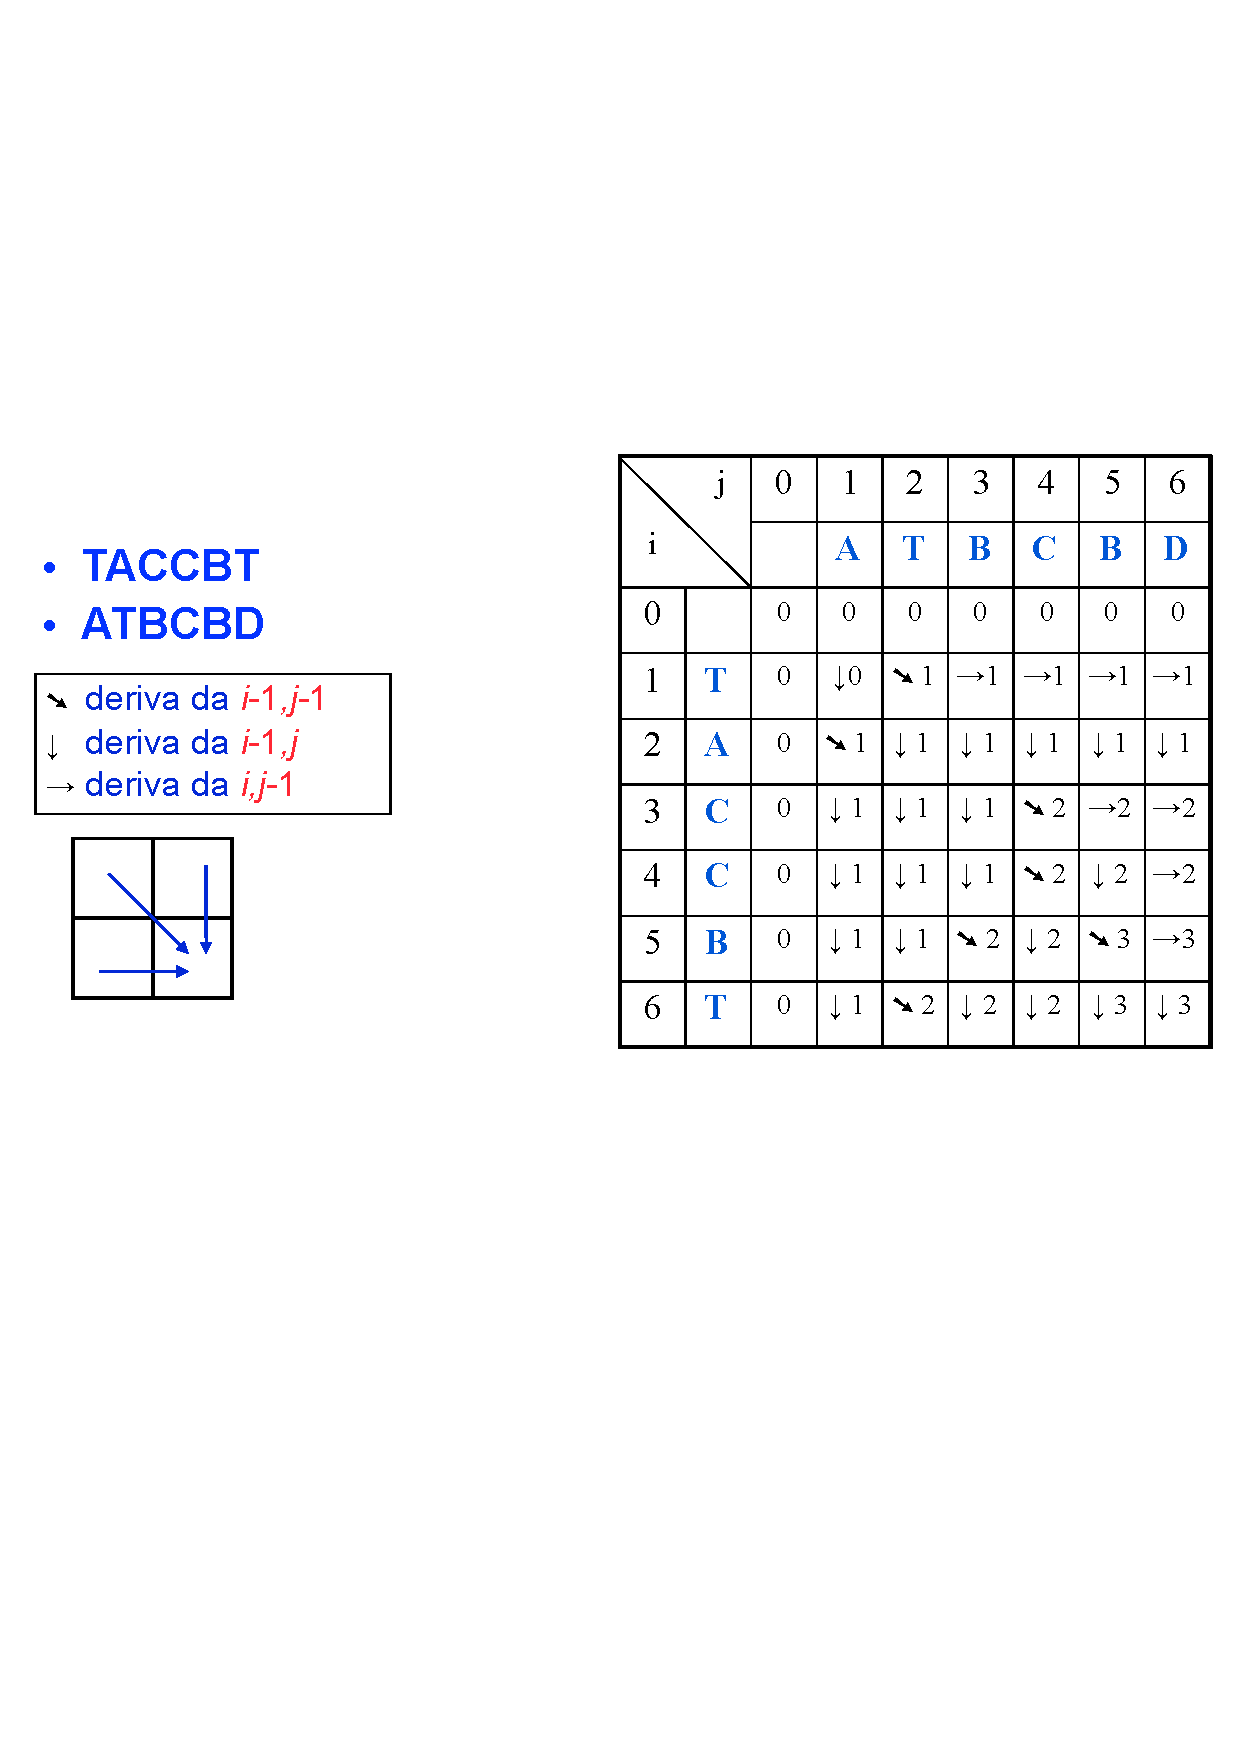
\includegraphics[width=0.95\textwidth,page=1]{lcs.pdf}

\tiny
\[
  \mathit{DP}[i][j] = \begin{cases}
   0 & i=0\ \OR\ j=0 \\
   \mathit{DP}[i-1][j-1]+1 & i>0\ \AND\ j>0\ \AND\ t_i = u_j \\
   \max \{ \mathit{DP}[i-1][j], \mathit{DP}[i][j-1] \} & i>0\ \AND\ j>0\ \AND\ t_i \neq u_j
  \end{cases}
\]

\end{frame}

% -----------------------------------------------------------------------------
\begin{frame}{Ricostruire la soluzione}

\centering
\vspace{-9pt}
\includegraphics[width=0.95\textwidth,page=2]{lcs.pdf}

\bigskip
\BB{Utilizzando la tabella, come possiamo ottenere la soluzione?}

\end{frame}


% -----------------------------------------------------------------------------
\begin{frame}[shrink=10]{Ricostruire la sottosequenza comune}

\vspace{-9pt}
\begin{Procedure}
\caption[A]{\INTEGER \LCS($\Item[\,]\ T,\ \Item[\,]\ U,\ \INTEGER\ n,\ \INTEGER\ m$)}
  $\ldots$\;
  \Return $\textsf{subsequence}(\mathit{DP}, T, U, n, m)$\;
\end{Procedure}

\vspace{-18pt}
\begin{Procedure}
\caption[A]{\List\ \textsf{subsequence}($\INTEGER[\,][\,]\ \mathit{DP}, \Item[\,]\ T,\ \Item[\,]\ U,\ \INTEGER\ i,\ \INTEGER\ j$)}
\If{$i \Eq 0$ \OR\ $j \Eq 0$}{
  \Return $\listconstructor()\;$
}
\eIf{$T[i] \Eq U[j]$}{
  $S = \textsf{subsequence}(\mathit{DP}, T, U, i-1, j-1)$\;
  $S.\listinsert(S.\listhead(), T[i])$\;
  \Return $S$\;
}{
  \eIf{$\mathit{DP}[i-1][j] > \mathit{DP}[i][j-1]$}{
    \Return $\textsf{subsequence}(\mathit{DP}, T, U, i-1, j)$\;
  }{
    \Return $\textsf{subsequence}(\mathit{DP}, T, U, i, j-1)$\;
  }
}
\end{Procedure}


\end{frame}

\begin{frame}{Complessità computazionale}

\vspace{-9pt}
\BB{Qual è la complessità computazionale di \textsf{subsequence()}?}

\pause
\[
  T(n) = O(m+n)
\]
  
\bigskip
\BB{Qual è la complessità computazionale di \textsf{LCS()}?}

\pause
\[
  T(n) = O(mn)
\]

\end{frame}

\begin{frame}[shrink=10]{Misura di similitudine}

\vspace{-9pt}
\BB{
Se si vuole solo misurare la lunghezza della LCS senza ricostruire la soluzione, è possibile conservare solo la riga precedente.
}

\vspace{-9pt}
\small
\begin{Procedure}
\caption[A]{\INTEGER \LCS($\Item[\,]\ T,\ \Item[\,]\ U,\ \INTEGER\ n,\ \INTEGER\ m$)}
$\INTARRAY[\,]\ \mathit{DP'} = \NEW\ \INTEGER[0 \ldots m] $\;
$\INTARRAY[\,]\ \mathit{DP} = \NEW\ \INTEGER[0 \ldots m]$\;
\For{$j = 0$ \TO $m$}{
  $\mathit{DP}[j] = 0$\;
}
\For{$i = 1$ \TO\ $n$}{
  $\mathit{DP'}, \mathit{DP} = \mathit{DP}, \mathit{DP'}$\;
  $\mathit{DP}[0] = 0$\;
  \For{$j = 1$ \TO $m$}{
    \eIf{$T[i]  \Eq  U[j]$}{
      $\mathit{DP}[j] = \mathit{DP'}[j-1]+1$\;
    }{
      $\mathit{DP}[j] = \MAX(\mathit{DP'}[j], \mathit{DP}[j-1])$\;
    }
  }
}
\Return $\mathit{DP}[m]$\;

\end{Procedure}



\end{frame}

\begin{frame}{Commenti finali}

\vspace{-9pt}
\begin{myboxtitle}[Take-home message (prendi e porta a casa)]
Non sempre è necessario memorizzare informazioni aggiuntive per ricostruire la soluzione.
\end{myboxtitle}

\begin{myboxtitle}[Take-home message (prendi e porta a casa)]
Se non è necessario ricostruire la soluzione, è possibile risparmiare spazio conservando solo i dati ancora utili.
\end{myboxtitle}


\end{frame}

\begin{frame}{Reality check -- LCS e \texttt{diff}  }

\vspace{-9pt}
\BB{\texttt{diff}}
\BIL
\item Esamina due file di testo, evidenziondone le differenze a livello di riga. 
\item Lavorare \alert{a livello di riga} significa che i confronti fra simboli sono in realtà confronti fra righe, e che $n$ ed $m$ sono il numero di righe dei due file
\EIL

\BB{Ottimizzazioni}
\BIL
\item \texttt{diff} è utilizzato soprattutto per codice sorgente; è possibile applicare euristiche sulle righe iniziali e finali
\item Per distinguere le righe - utilizzo di funzioni hash
\EIL

\end{frame}

\begin{frame}{Reality check -- LCS e \texttt{diff}  }

\vspace{-9pt}
\IG{1.0}{diff.pdf}

\end{frame}


\end{document}




